\documentclass[10pt]{article}

\usepackage[utf8]{inputenc}
\usepackage{hyperref}
\usepackage{mathtools}
\usepackage{enumitem}
\urlstyle{sf}
\usepackage[margin=1in]{geometry}

\begin{document}

\begin{center}
{\LARGE\noindent Supplemental Material for: Predicting off-target binding
    profiles with confidence using Conformal Prediction}
\end{center}

Supplemental 1: Calibration plots for all targets. See figure
\ref{fig:calplots_all}.

\begin{figure}[h!]

\vspace*{-15pt} % This is cheating, top margin should be holy, but this table is HUGE!
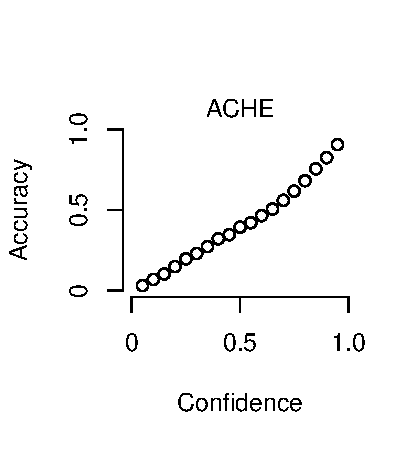
\includegraphics[width=0.19\textwidth]{figures/calibration_plots/ache_calib.pdf}
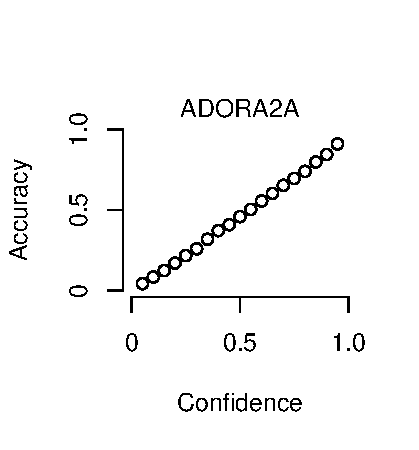
\includegraphics[width=0.19\textwidth]{figures/calibration_plots/adora2a_calib.pdf}
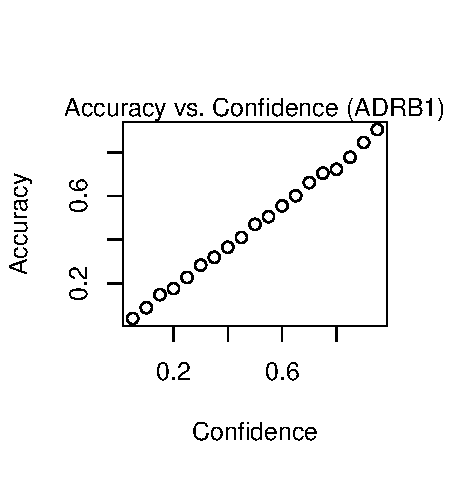
\includegraphics[width=0.19\textwidth]{figures/calibration_plots/adrb1_calib.pdf}
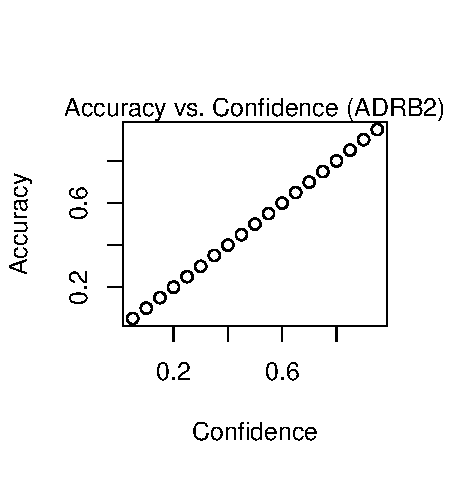
\includegraphics[width=0.19\textwidth]{figures/calibration_plots/adrb2_calib.pdf}
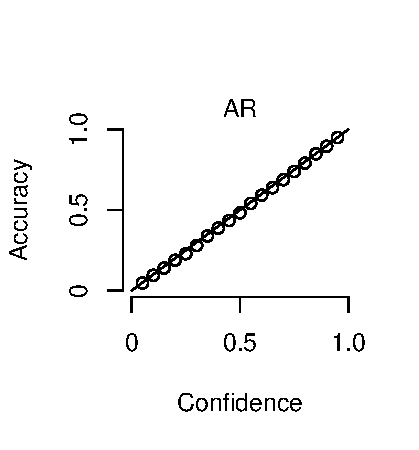
\includegraphics[width=0.19\textwidth]{figures/calibration_plots/ar_calib.pdf}
\vspace*{-15pt} % This is cheating, top margin should be holy, but this table is HUGE!
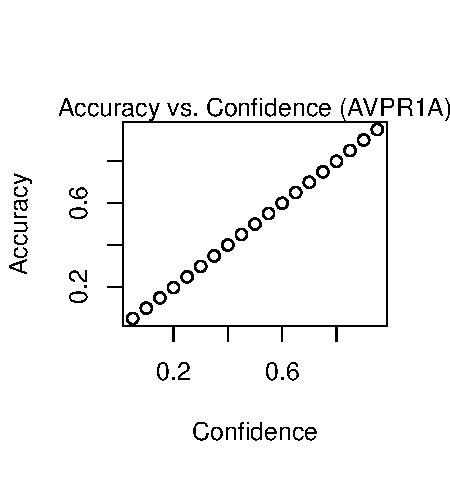
\includegraphics[width=0.19\textwidth]{figures/calibration_plots/avpr1a_calib.pdf}
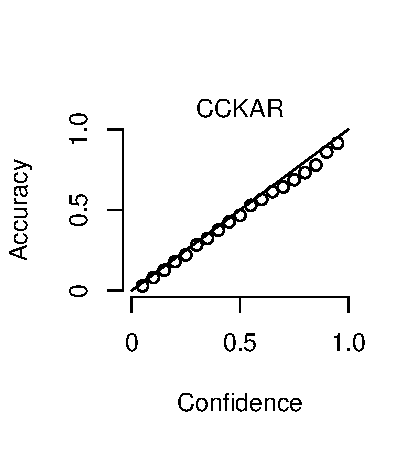
\includegraphics[width=0.19\textwidth]{figures/calibration_plots/cckar_calib.pdf}
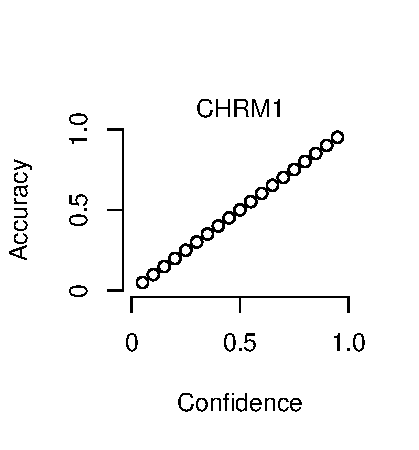
\includegraphics[width=0.19\textwidth]{figures/calibration_plots/chrm1_calib.pdf}
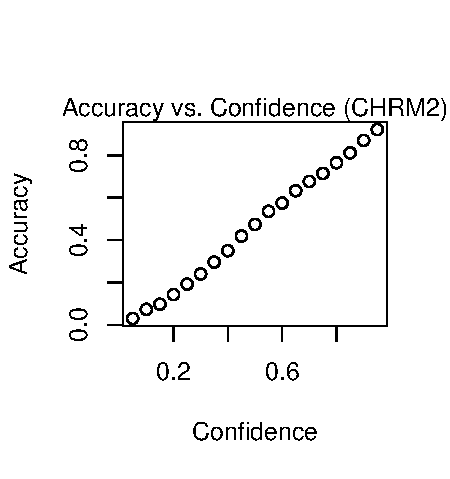
\includegraphics[width=0.19\textwidth]{figures/calibration_plots/chrm2_calib.pdf}
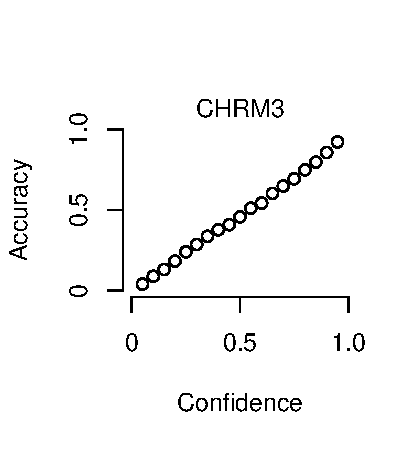
\includegraphics[width=0.19\textwidth]{figures/calibration_plots/chrm3_calib.pdf}
\vspace*{-15pt} % This is cheating, top margin should be holy, but this table is HUGE!
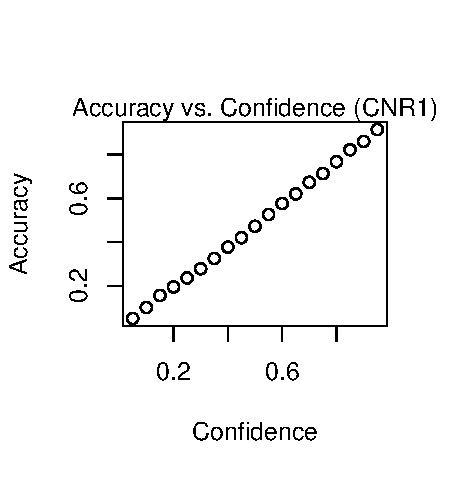
\includegraphics[width=0.19\textwidth]{figures/calibration_plots/cnr1_calib.pdf}
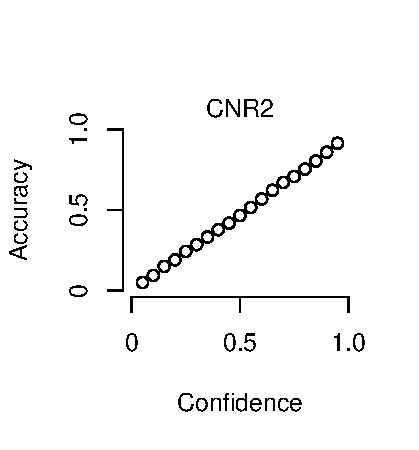
\includegraphics[width=0.19\textwidth]{figures/calibration_plots/cnr2_calib.pdf}
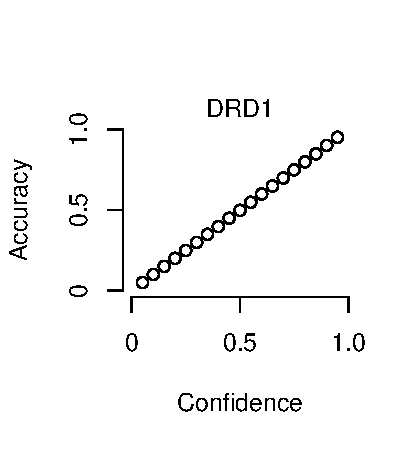
\includegraphics[width=0.19\textwidth]{figures/calibration_plots/drd1_calib.pdf}
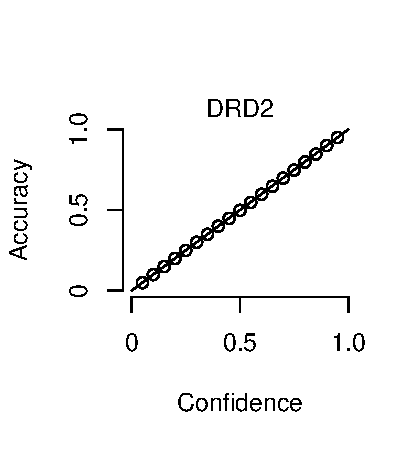
\includegraphics[width=0.19\textwidth]{figures/calibration_plots/drd2_calib.pdf}
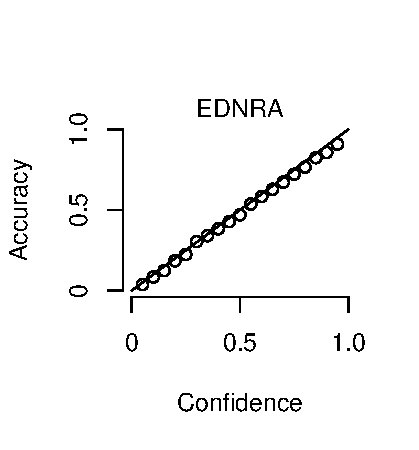
\includegraphics[width=0.19\textwidth]{figures/calibration_plots/ednra_calib.pdf}
\vspace*{-15pt} % This is cheating, top margin should be holy, but this table is HUGE!
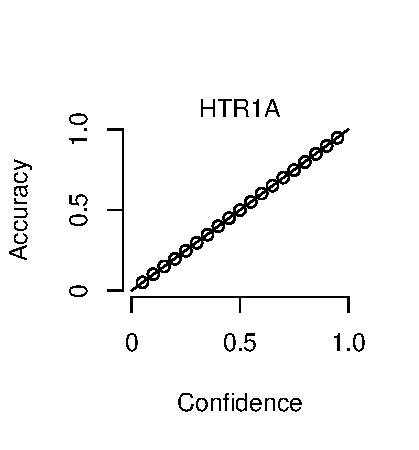
\includegraphics[width=0.19\textwidth]{figures/calibration_plots/htr1a_calib.pdf}
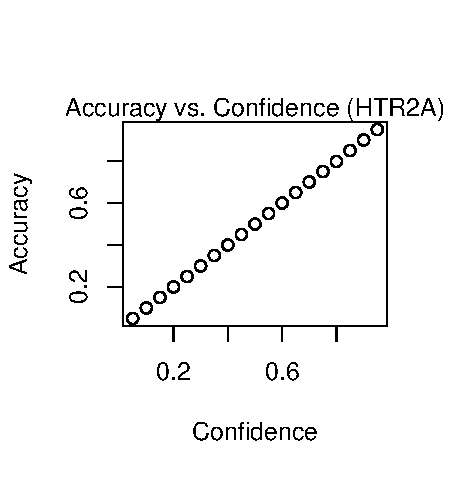
\includegraphics[width=0.19\textwidth]{figures/calibration_plots/htr2a_calib.pdf}
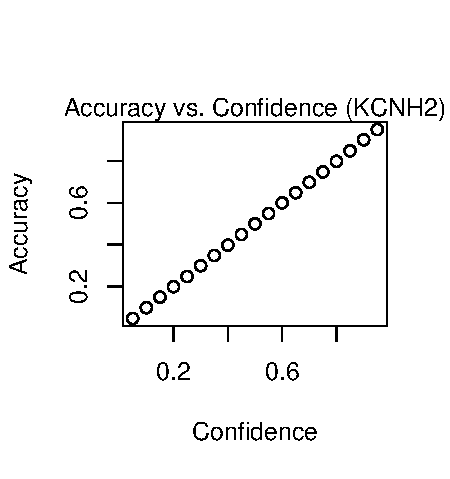
\includegraphics[width=0.19\textwidth]{figures/calibration_plots/kcnh2_calib.pdf}
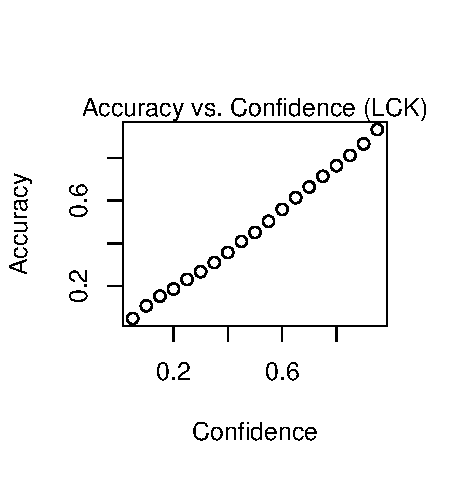
\includegraphics[width=0.19\textwidth]{figures/calibration_plots/lck_calib.pdf}
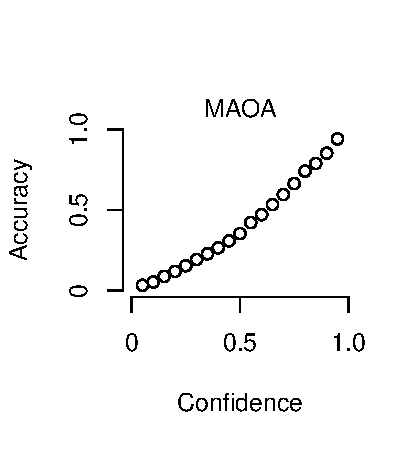
\includegraphics[width=0.19\textwidth]{figures/calibration_plots/maoa_calib.pdf}
\vspace*{-15pt} % This is cheating, top margin should be holy, but this table is HUGE!
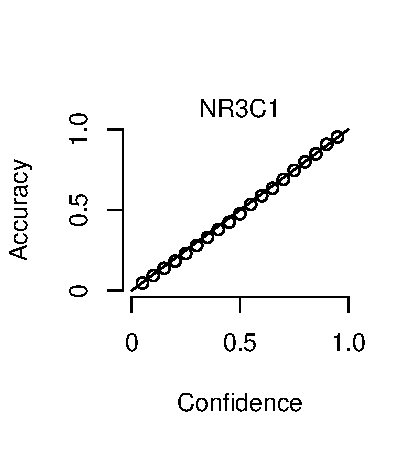
\includegraphics[width=0.19\textwidth]{figures/calibration_plots/nr3c1_calib.pdf}
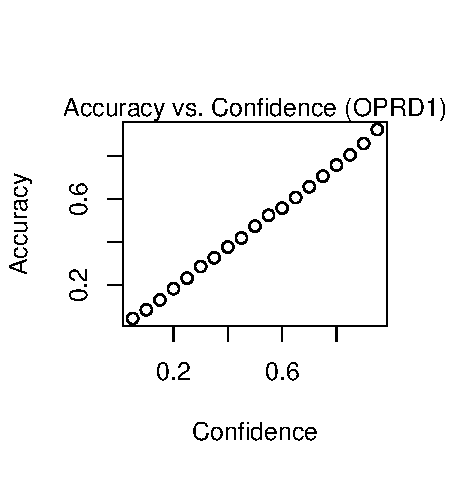
\includegraphics[width=0.19\textwidth]{figures/calibration_plots/oprd1_calib.pdf}
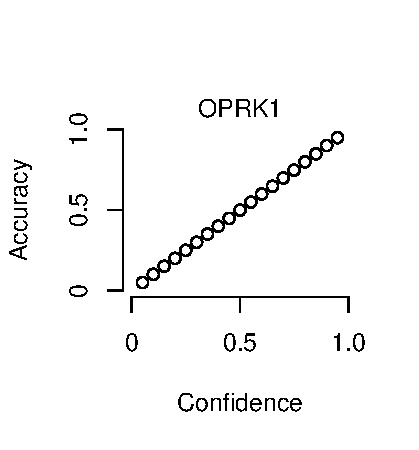
\includegraphics[width=0.19\textwidth]{figures/calibration_plots/oprk1_calib.pdf}
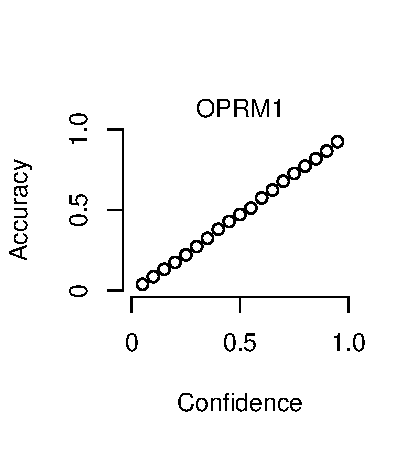
\includegraphics[width=0.19\textwidth]{figures/calibration_plots/oprm1_calib.pdf}
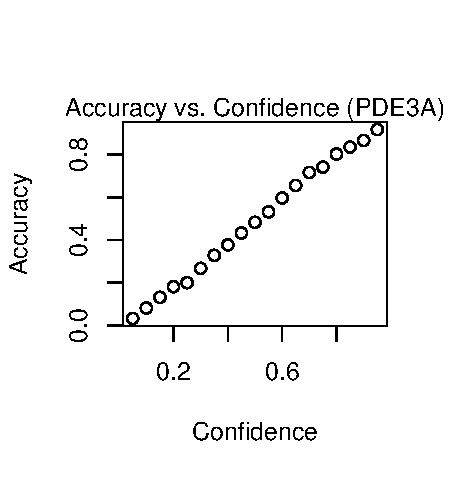
\includegraphics[width=0.19\textwidth]{figures/calibration_plots/pde3a_calib.pdf}
\vspace*{-15pt} % This is cheating, top margin should be holy, but this table is HUGE!
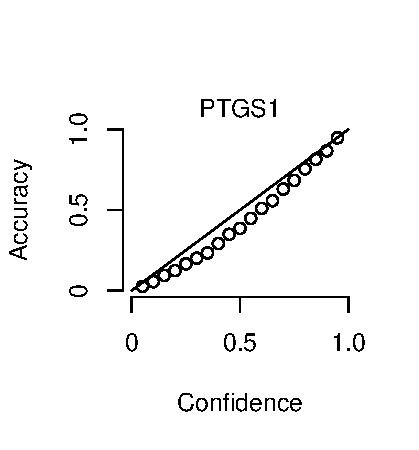
\includegraphics[width=0.19\textwidth]{figures/calibration_plots/ptgs1_calib.pdf}
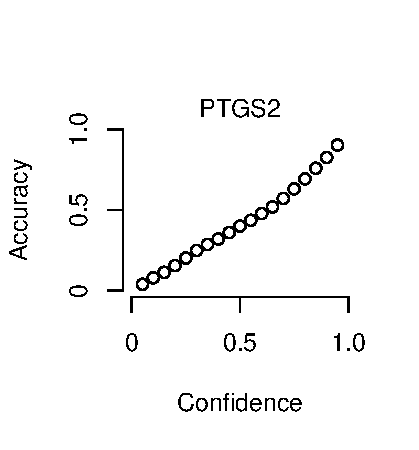
\includegraphics[width=0.19\textwidth]{figures/calibration_plots/ptgs2_calib.pdf}
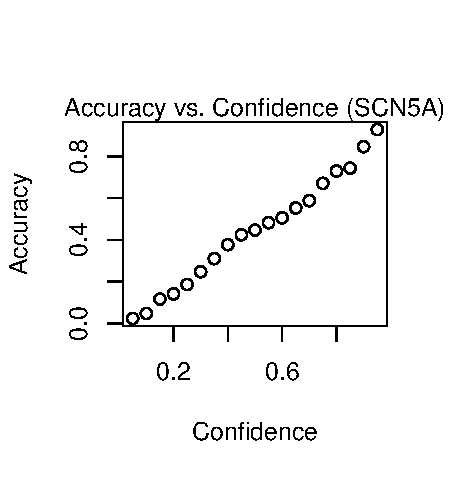
\includegraphics[width=0.19\textwidth]{figures/calibration_plots/scn5a_calib.pdf}
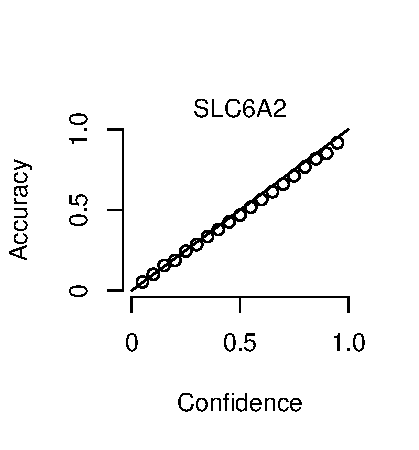
\includegraphics[width=0.19\textwidth]{figures/calibration_plots/slc6a2_calib.pdf}
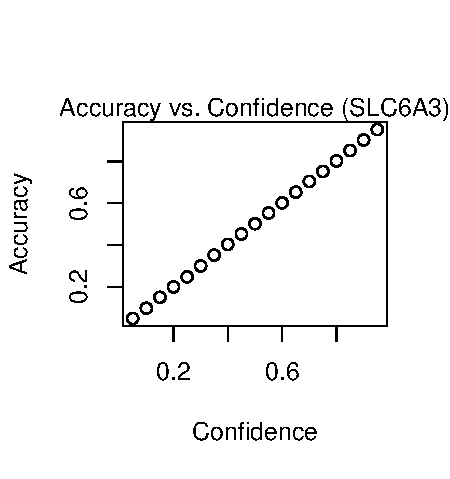
\includegraphics[width=0.19\textwidth]{figures/calibration_plots/slc6a3_calib.pdf}
\vspace*{-15pt} % This is cheating, top margin should be holy, but this table is HUGE!
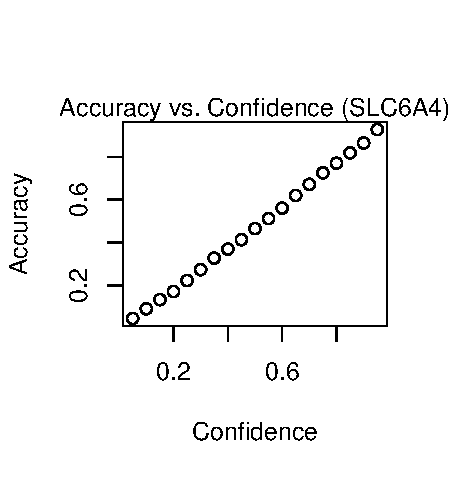
\includegraphics[width=0.19\textwidth]{figures/calibration_plots/slc6a4_calib.pdf}
    \caption{Calibration plots for all targets. The plots show accuracy against
        confidence, for confidence values 0.05 to 0.95 with a step size of 0.05.}
    \label{fig:calplots_all}
\end{figure}

Supplemental 2: Predicted versus observed labels, at confidence level 0.8,
    for all targets \ref{fig:valplots_all_0.8}.

\begin{figure}[h!]

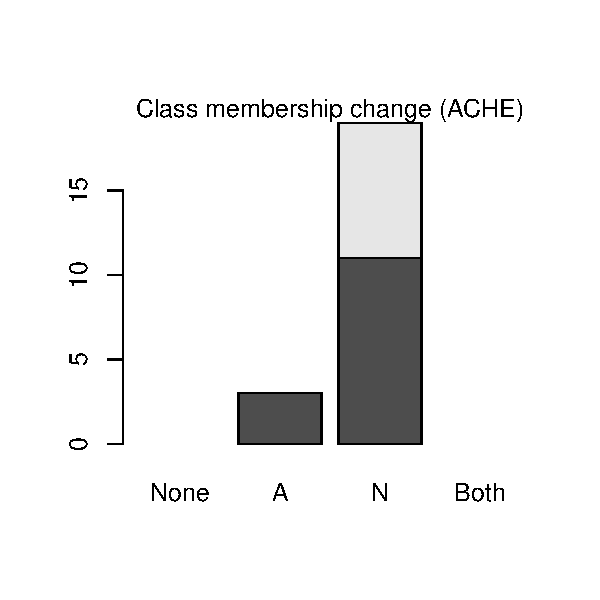
\includegraphics[width=0.15\textwidth]{figures/validation_plots/ache_0p8_valplot.pdf}
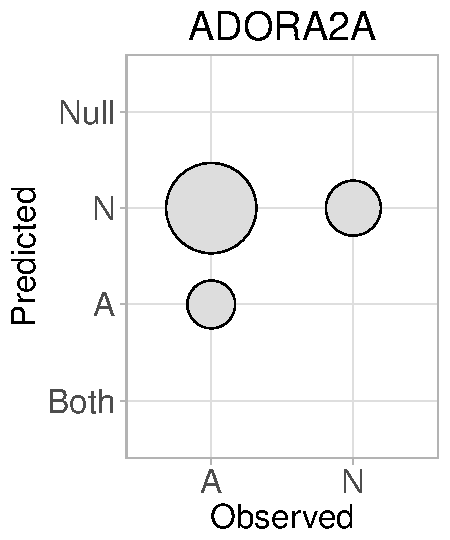
\includegraphics[width=0.15\textwidth]{figures/validation_plots/adora2a_0p8_valplot.pdf}
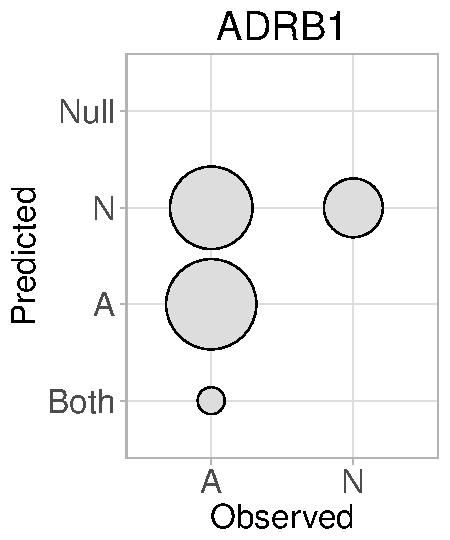
\includegraphics[width=0.15\textwidth]{figures/validation_plots/adrb1_0p8_valplot.pdf}
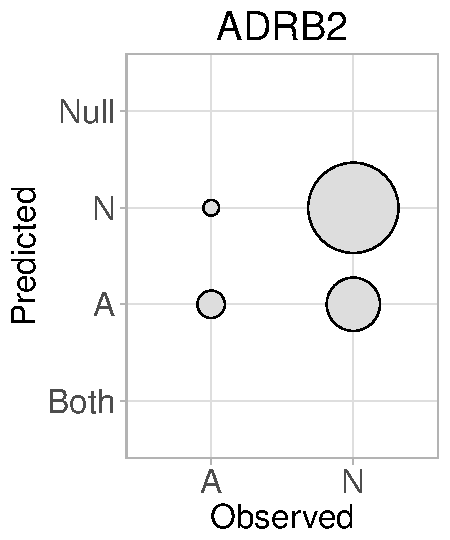
\includegraphics[width=0.15\textwidth]{figures/validation_plots/adrb2_0p8_valplot.pdf}
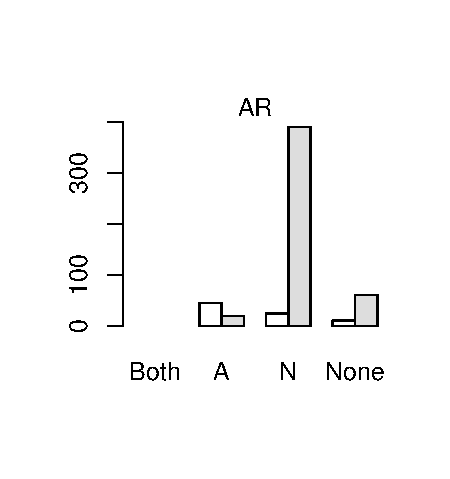
\includegraphics[width=0.15\textwidth]{figures/validation_plots/ar_0p8_valplot.pdf}
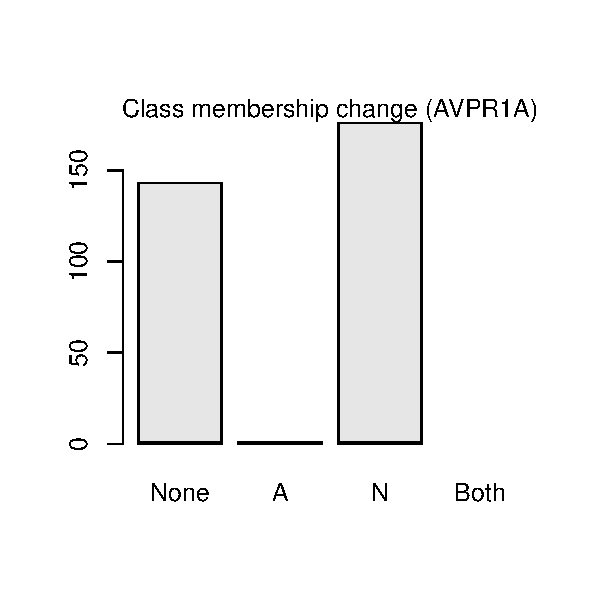
\includegraphics[width=0.15\textwidth]{figures/validation_plots/avpr1a_0p8_valplot.pdf}
\vspace*{10pt} % This is cheating, top margin should be holy, but this table is HUGE!
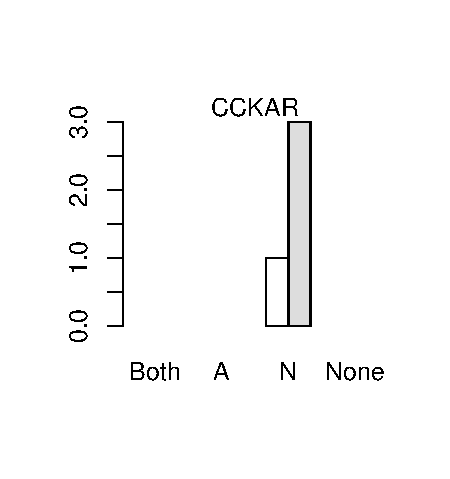
\includegraphics[width=0.15\textwidth]{figures/validation_plots/cckar_0p8_valplot.pdf}
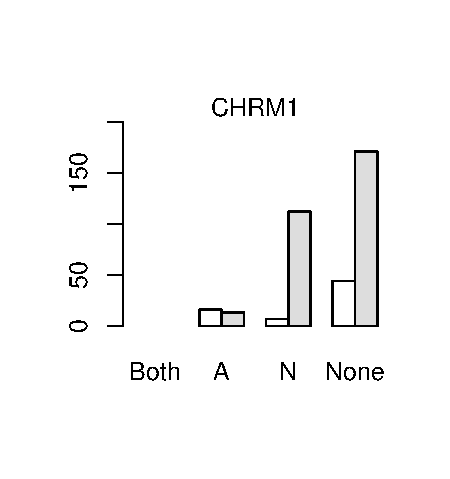
\includegraphics[width=0.15\textwidth]{figures/validation_plots/chrm1_0p8_valplot.pdf}
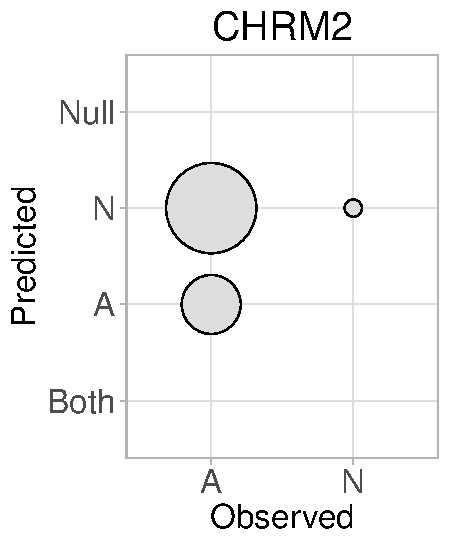
\includegraphics[width=0.15\textwidth]{figures/validation_plots/chrm2_0p8_valplot.pdf}
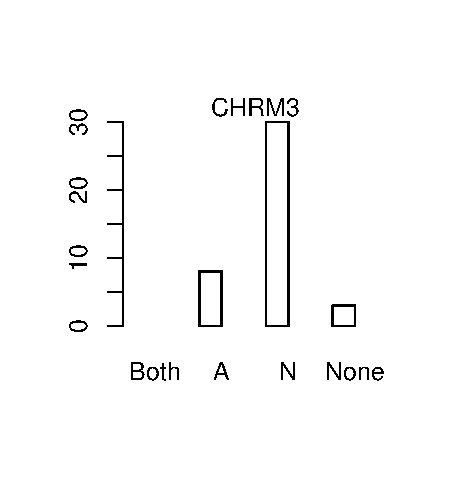
\includegraphics[width=0.15\textwidth]{figures/validation_plots/chrm3_0p8_valplot.pdf}
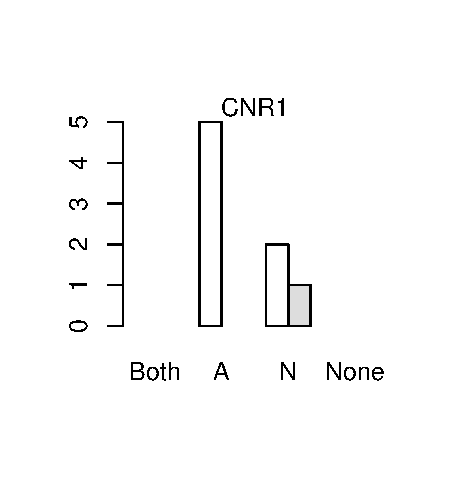
\includegraphics[width=0.15\textwidth]{figures/validation_plots/cnr1_0p8_valplot.pdf}
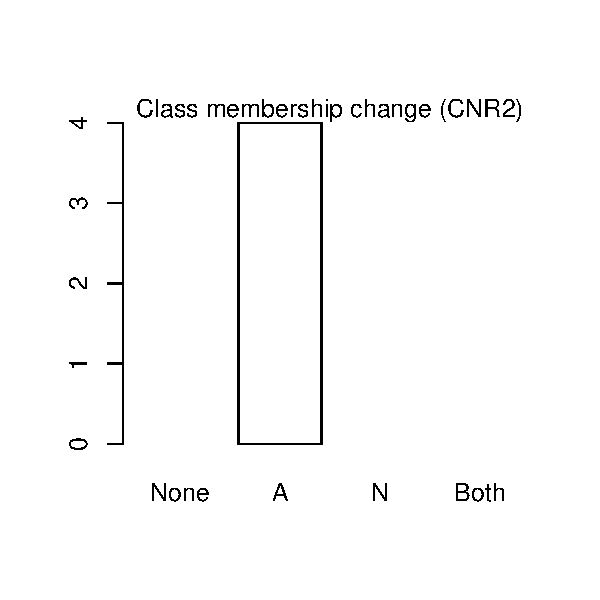
\includegraphics[width=0.15\textwidth]{figures/validation_plots/cnr2_0p8_valplot.pdf}
\vspace*{10pt} % This is cheating, top margin should be holy, but this table is HUGE!
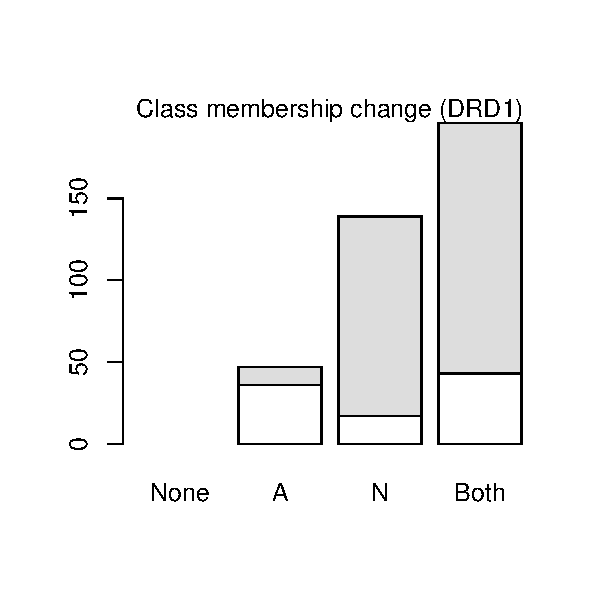
\includegraphics[width=0.15\textwidth]{figures/validation_plots/drd1_0p8_valplot.pdf}
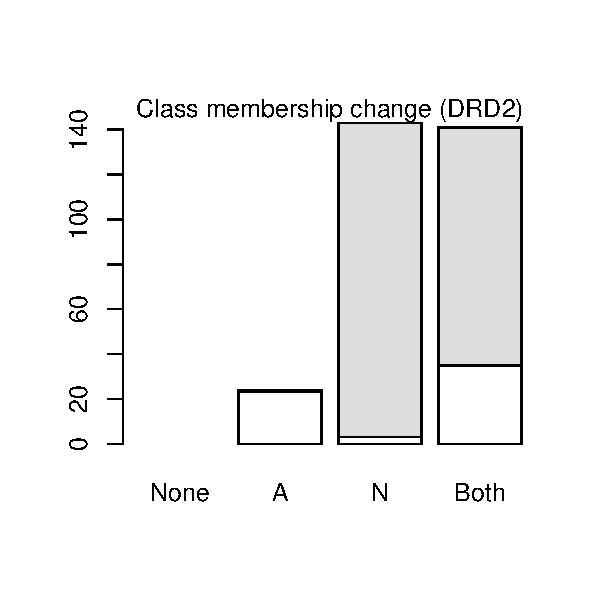
\includegraphics[width=0.15\textwidth]{figures/validation_plots/drd2_0p8_valplot.pdf}
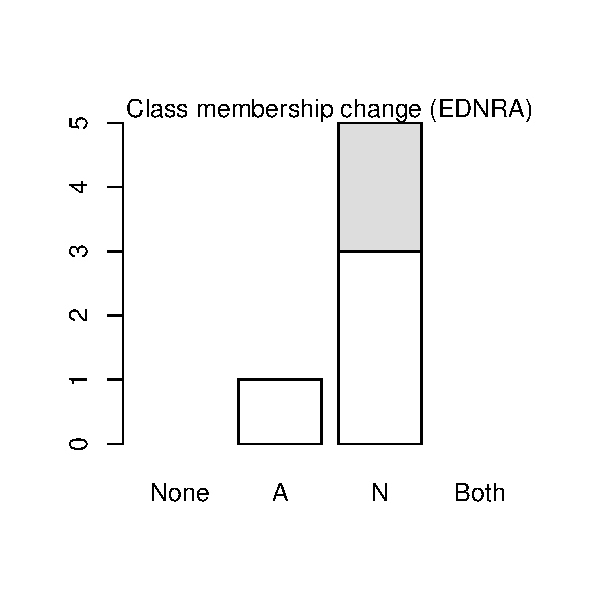
\includegraphics[width=0.15\textwidth]{figures/validation_plots/ednra_0p8_valplot.pdf}
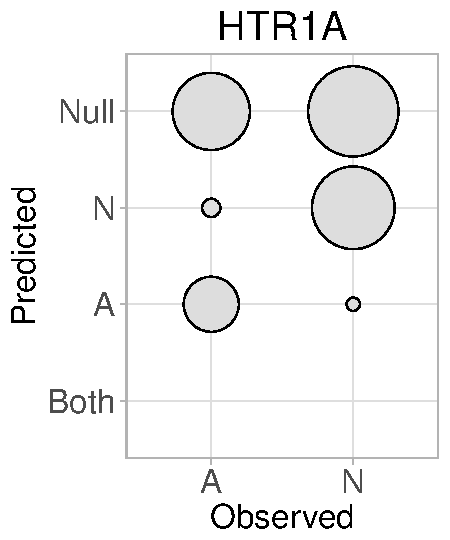
\includegraphics[width=0.15\textwidth]{figures/validation_plots/htr1a_0p8_valplot.pdf}
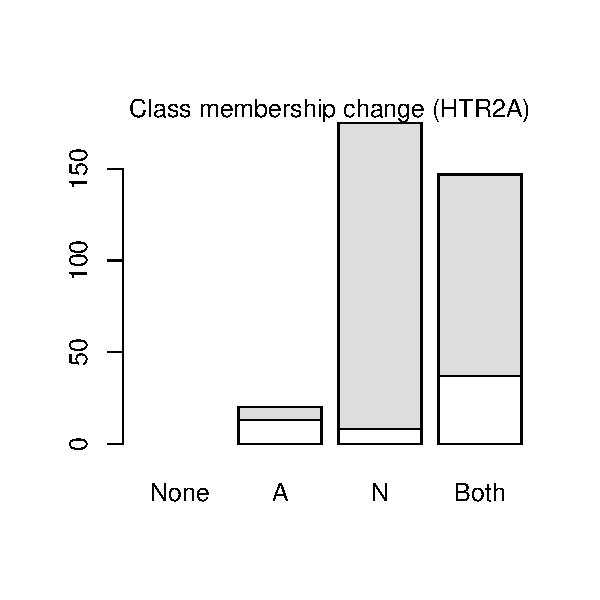
\includegraphics[width=0.15\textwidth]{figures/validation_plots/htr2a_0p8_valplot.pdf}
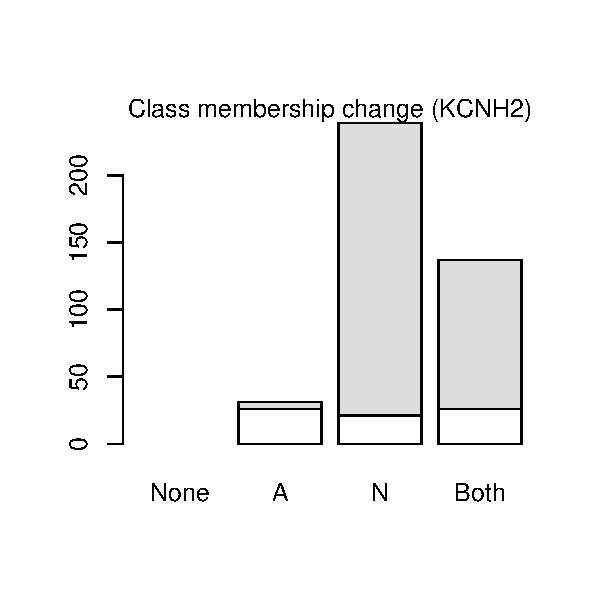
\includegraphics[width=0.15\textwidth]{figures/validation_plots/kcnh2_0p8_valplot.pdf}
\vspace*{10pt} % This is cheating, top margin should be holy, but this table is HUGE!
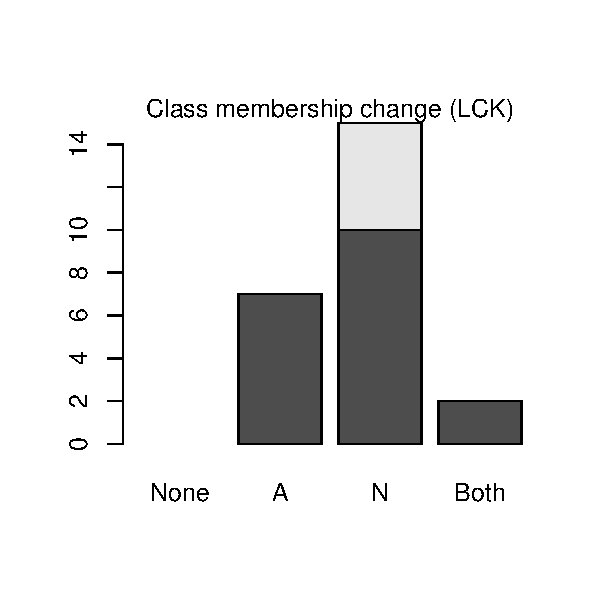
\includegraphics[width=0.15\textwidth]{figures/validation_plots/lck_0p8_valplot.pdf}
\includegraphics[width=0.15\textwidth]{figures/validation_plots/maoa_0p8_valplot.pdf}
\includegraphics[width=0.15\textwidth]{figures/validation_plots/nr3c1_0p8_valplot.pdf}
\includegraphics[width=0.15\textwidth]{figures/validation_plots/oprd1_0p8_valplot.pdf}
\includegraphics[width=0.15\textwidth]{figures/validation_plots/oprk1_0p8_valplot.pdf}
\includegraphics[width=0.15\textwidth]{figures/validation_plots/oprm1_0p8_valplot.pdf}
\vspace*{10pt} % This is cheating, top margin should be holy, but this table is HUGE!
\includegraphics[width=0.15\textwidth]{figures/validation_plots/pde3a_0p8_valplot.pdf}
\includegraphics[width=0.15\textwidth]{figures/validation_plots/ptgs1_0p8_valplot.pdf}
\includegraphics[width=0.15\textwidth]{figures/validation_plots/ptgs2_0p8_valplot.pdf}
\includegraphics[width=0.15\textwidth]{figures/validation_plots/scn5a_0p8_valplot.pdf}
\includegraphics[width=0.15\textwidth]{figures/validation_plots/slc6a2_0p8_valplot.pdf}
\includegraphics[width=0.15\textwidth]{figures/validation_plots/slc6a3_0p8_valplot.pdf}
\vspace*{10pt} % This is cheating, top margin should be holy, but this table is HUGE!
\includegraphics[width=0.15\textwidth]{figures/validation_plots/slc6a4_0p8_valplot.pdf}

    \caption{Predicted versus observed labels, at confidence level 0.8,
    for all targets, and all compounds in the prediction dataset.
    The X-axis represents observed labels, as found in ExcapeDB, while Y-axis
    shows predicted labels. The areas of the circles is proportional to the
    number of compounds per predicted/observed combination. Note that the scale
    is different between each plot, because of differing total number of
    compounds per target.}
    \label{fig:valplots_all_0.8}
\end{figure}

Supplemental 3: Predicted versus observed labels, at confidence level 0.9,
    for all targets \ref{fig:valplots_all_0.9}.

\begin{figure}[h!]

\includegraphics[width=0.15\textwidth]{figures/validation_plots/ache_0p9_valplot.pdf}
\includegraphics[width=0.15\textwidth]{figures/validation_plots/adora2a_0p9_valplot.pdf}
\includegraphics[width=0.15\textwidth]{figures/validation_plots/adrb1_0p9_valplot.pdf}
\includegraphics[width=0.15\textwidth]{figures/validation_plots/adrb2_0p9_valplot.pdf}
\includegraphics[width=0.15\textwidth]{figures/validation_plots/ar_0p9_valplot.pdf}
\includegraphics[width=0.15\textwidth]{figures/validation_plots/avpr1a_0p9_valplot.pdf}
\vspace*{10pt} % This is cheating, top margin should be holy, but this table is HUGE!
\includegraphics[width=0.15\textwidth]{figures/validation_plots/cckar_0p9_valplot.pdf}
\includegraphics[width=0.15\textwidth]{figures/validation_plots/chrm1_0p9_valplot.pdf}
\includegraphics[width=0.15\textwidth]{figures/validation_plots/chrm2_0p9_valplot.pdf}
\includegraphics[width=0.15\textwidth]{figures/validation_plots/chrm3_0p9_valplot.pdf}
\includegraphics[width=0.15\textwidth]{figures/validation_plots/cnr1_0p9_valplot.pdf}
\includegraphics[width=0.15\textwidth]{figures/validation_plots/cnr2_0p9_valplot.pdf}
\vspace*{10pt} % This is cheating, top margin should be holy, but this table is HUGE!
\includegraphics[width=0.15\textwidth]{figures/validation_plots/drd1_0p9_valplot.pdf}
\includegraphics[width=0.15\textwidth]{figures/validation_plots/drd2_0p9_valplot.pdf}
\includegraphics[width=0.15\textwidth]{figures/validation_plots/ednra_0p9_valplot.pdf}
\includegraphics[width=0.15\textwidth]{figures/validation_plots/htr1a_0p9_valplot.pdf}
\includegraphics[width=0.15\textwidth]{figures/validation_plots/htr2a_0p9_valplot.pdf}
\includegraphics[width=0.15\textwidth]{figures/validation_plots/kcnh2_0p9_valplot.pdf}
\vspace*{10pt} % This is cheating, top margin should be holy, but this table is HUGE!
\includegraphics[width=0.15\textwidth]{figures/validation_plots/lck_0p9_valplot.pdf}
\includegraphics[width=0.15\textwidth]{figures/validation_plots/maoa_0p9_valplot.pdf}
\includegraphics[width=0.15\textwidth]{figures/validation_plots/nr3c1_0p9_valplot.pdf}
\includegraphics[width=0.15\textwidth]{figures/validation_plots/oprd1_0p9_valplot.pdf}
\includegraphics[width=0.15\textwidth]{figures/validation_plots/oprk1_0p9_valplot.pdf}
\includegraphics[width=0.15\textwidth]{figures/validation_plots/oprm1_0p9_valplot.pdf}
\vspace*{10pt} % This is cheating, top margin should be holy, but this table is HUGE!
\includegraphics[width=0.15\textwidth]{figures/validation_plots/pde3a_0p9_valplot.pdf}
\includegraphics[width=0.15\textwidth]{figures/validation_plots/ptgs1_0p9_valplot.pdf}
\includegraphics[width=0.15\textwidth]{figures/validation_plots/ptgs2_0p9_valplot.pdf}
\includegraphics[width=0.15\textwidth]{figures/validation_plots/scn5a_0p9_valplot.pdf}
\includegraphics[width=0.15\textwidth]{figures/validation_plots/slc6a2_0p9_valplot.pdf}
\includegraphics[width=0.15\textwidth]{figures/validation_plots/slc6a3_0p9_valplot.pdf}
\vspace*{10pt} % This is cheating, top margin should be holy, but this table is HUGE!
\includegraphics[width=0.15\textwidth]{figures/validation_plots/slc6a4_0p9_valplot.pdf}

    \caption{Predicted versus observed labels, at confidence level 0.9,
    for all targets, and all compounds in the prediction dataset.
    The X-axis represents observed labels, as found in ExcapeDB, while Y-axis
    shows predicted labels. The areas of the circles is proportional to the
    number of compounds per predicted/observed combination. Note that the scale
    is different between each plot, because of differing total number of
    compounds per target.}
    \label{fig:valplots_all_0.9}
\end{figure}

Supplemental 4: Detailed workflow graphs.

Detailed workflow graph for the comparing the effect of extending target
datasets with assumed non-actives, can be seen in figure
\ref{fig:workflow_detailed_fillup_vs_not}.

Detailed workflow graph for the workflow where DrugBank compounds were removed,
can be seen in figure~\ref{fig:workflow_detailed_wo_drugbank}.

\begin{figure}[h!]
\includegraphics[width=\textwidth]{figures/workflow_graph_fillup_vs_not.pdf}
    \caption{Detailed workflow graph for comparing the effect of extending
    target datasets with assumed non-actives.}
    \label{fig:workflow_detailed_fillup_vs_not}
\end{figure}

\begin{figure}[h!]
\includegraphics[width=\textwidth]{figures/workflow_graph_wo_drugbank.pdf}
    \caption{Detailed workflow graph for the workflow where DrugBank compounds
    were removed. Note the additional components in the top of the figure, for
    preparing and extracting data from the DrugBank dataset.}
    \label{fig:workflow_detailed_wo_drugbank}
\end{figure}

\end{document}


